Dieses Kapitel setzt voraus, dass Traverso \Version\ oder neuer auf dem System installiert ist. Falls dies nicht der Fall ist, sollte zunächst die Installation wie in Kapitel \ref{sect_installation} beschrieben durchgeführt werden.

Startet Traverso vom Programmemenü oder durch drücken von Alt+F2 und Eingabe von \texttt{traverso}. Als erstes werdet ihr nach dem Projektverzeichnis gefragt. Falls es noch nicht existiert, erstell in diesem Dialog ein neues. Das Projektverzeichnis wird alle Projekte inklusive der aufgenommenen Audiodateien enthalten. Falls ihr also ernsthaft mit Traverso arbeiten wollt, solltet ihr es mit Bedacht auswählen, da schnell einige Gigabytes an Audiodaten anfallen können. Wechselt nun in das gewünschte Verzeichnis und drückt OK. Traverso bestätigt noch einmal die Auswahl, und startet dann das Hauptfenster. Dieses besteht aus verschiedenen Regionen, die alle sensitiv für weiche Selektion sind. Die Nomenklatur (\FigB\ \ref{fig_gui01}) wird in diesem Handbuch weitgehend auf Englisch beibehalten, um Verwirrung bei der Kommunikation in englischsprachigen Online-Quellen vorzubeugen. Für gängige Begriffe wird jedoch manchmal auch der deutsche Ausdruck verwendet (z.\,B. ,,Track'' und ,,Spur'' sind gleichwertig).

\begin{figure}
 \centering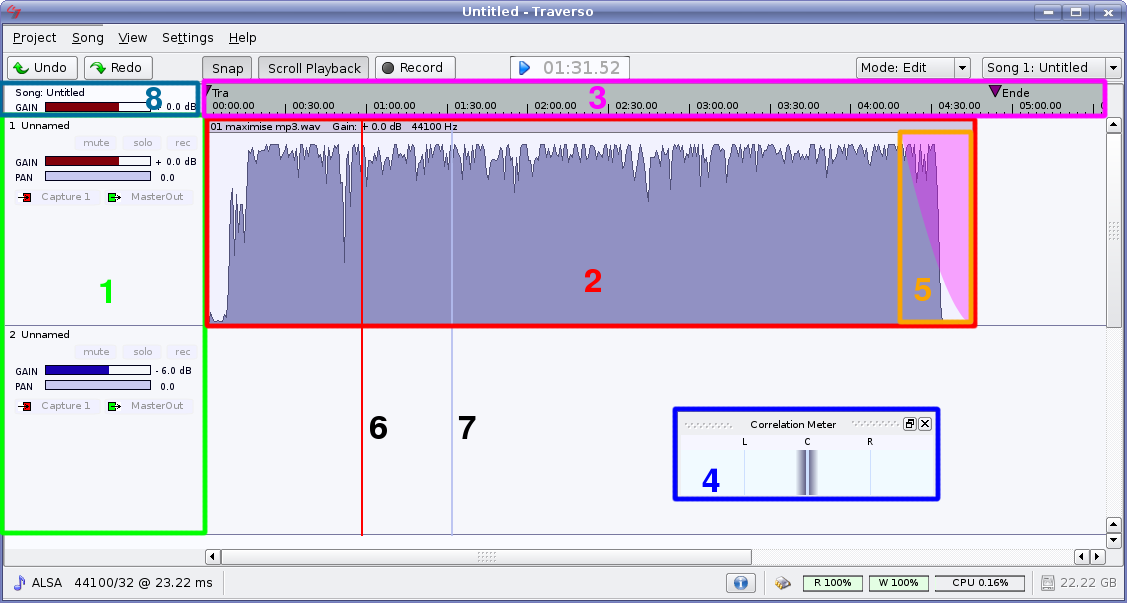
\includegraphics[width=\textwidth]{images/sshot06.png}
 \caption{Elemente der Benutzerschnittstelle von Traverso: 1 Track panel: Befindet sich der Mauszeiger darüber, empfängt es alle Tastenaktionen; 2 Audio clip: empfängt ebenfalls alle Tastenaktionen; 3 Time line (Zeitachse): Tastenaktionen werden von den Markern in der Zeitachse empfangen; 4 Dock window / Dock widget; 5 Fade out (Ausblenden); 6 Work cursor (Arbeitscursor); 7 Play head (Abspielcursor); 8 Sheet area.}
 \label{fig_gui01}
\end{figure}

Traverso verwendet sogenannte Dock-Fenster für viele Werkzeuge, die vom Hauptfenster abgelöst und frei plaziert werden können, indem man sie an ihrer Titelleiste herauszieht. Sie können auch übereinander gestapelt werden, oder frei schwebend auf einen zweiten Bildschirm verschoben werden (\FigB\ \ref{fig_mainwin02}).

\begin{figure}
 \centering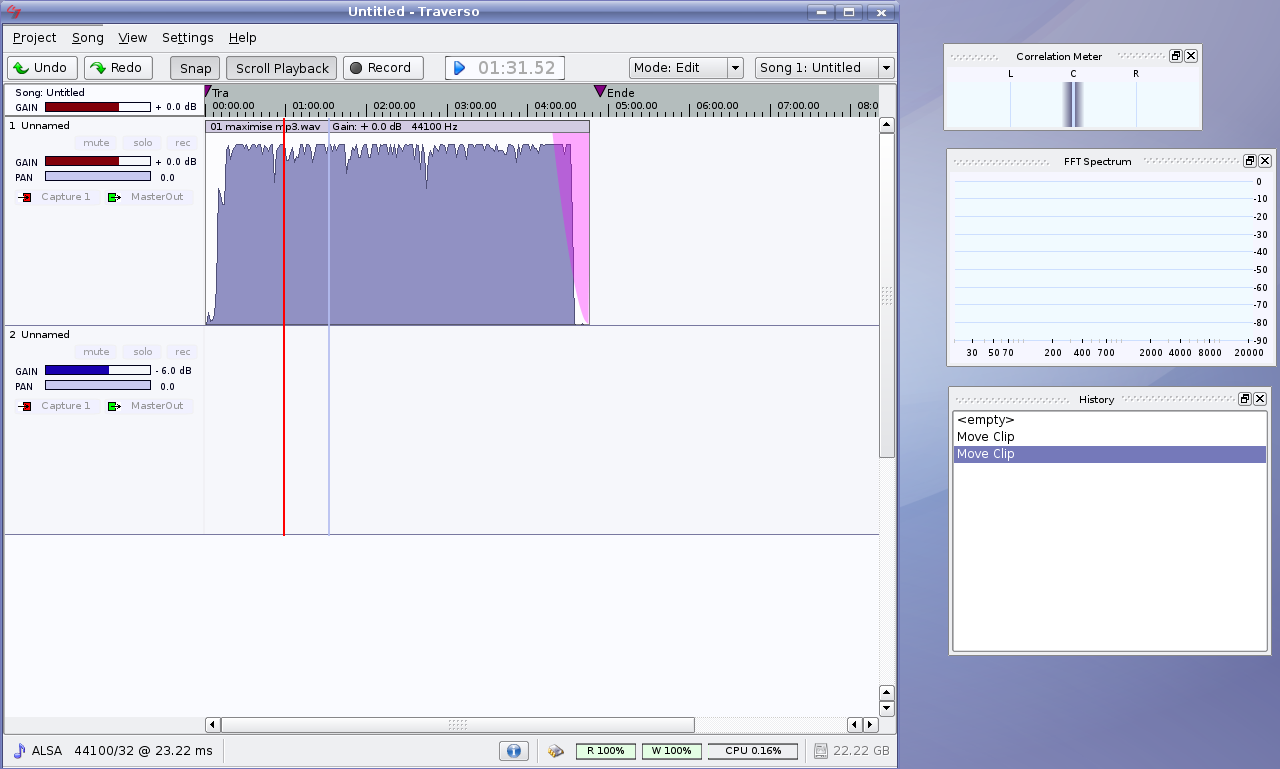
\includegraphics[width=0.9\textwidth]{images/sshot03.png}
 \caption{Die Dock-Fenster können vom Hauptfenster gelöst und frei plaziert werden. Dies ist besonders für Arbeitsplätze mit mehreren Bildschirmen interessant.}
 \label{fig_mainwin02}
\end{figure}

\section{Das Treiber-Backend}
Zur Zeit werden vier Treiber-Systeme unterstützt: Der Null-Treiber, ALSA, Jack, und Port Audio, letzteres als Schnittstelle zu WDM auf Windows und CoreAudio auf Mac OS X. Die einzelnen Treiber und ihre Einrichtung werden im Folgenden kurz besprochen. Der aktuell geladene Treiber wird in der unteren Menüleiste angezeigt.

\subsection{Null-Treiber}

\includegraphics[height=\baselineskip]{images/tux.png}

\includegraphics[height=\baselineskip]{images/mac.png}

\includegraphics[height=\baselineskip]{images/win.png}
\\
Dieser Treiber hat eigentlich keine Funktion und wird nur geladen, wenn kein anderer Treiber verfügbar ist. Es ist jedoch nicht möglich, über diesen Treiber Audiosignale abzuspielen oder aufzunehmen. Wird der Null-Treiber geladen, sollte man als erstes versuchen, einen der anderen Treiber zu aktivieren. Dazu klickt man auf den Eintrag in der unteren Menüleiste, um den Dialog in \FigT\ \ref{fig_driverconf} zu öffnen.

\subsection{ALSA}

\includegraphics[height=\baselineskip]{images/tux.png}
\\
Wird der ALSA-Treiber gestartet (auf Linux), kommuniziert Traverso direkt mit der ALSA-Schicht. Dies ist jedoch nur möglich, wenn keine andere Anwendung auf ALSA zugreift. Deshalb sollten vorher alle anderen Sound- oder Multimedia-Anwendungen gestoppt werden, und es muss sichergestellt werden, dass keine Soundserver (z.\,B. aRTs von KDE) aktiv sind. Anschlie"send kann ALSA in Traverso aktiviert werden, zunächst am besten mit einer Samplerate von 44100 Hz und einer Latenzzeit im Bereich von 11 bis 44~ms. Diese Werte können natürlich den Bedürfnissen und der Leistungsfähigkeit der Hardware angepasst werden. (Weitere Einstellungen können im Menü ,,Einstellungen $\rightarrow$ Einstellungen\dots $\rightarrow$ Audio Treiber'' vorgenommen werden.) Nach drücken von OK sollte der Eintrag in der Menüleiste von ,,Null-Treiber'' auf ,,ALSA'' wechseln. Tut er dies nicht, ist vermutlich noch eine Anwendung aktiv, die ALSA blockiert.

\subsection{Jack}

\includegraphics[height=\baselineskip]{images/tux.png}

\includegraphics[height=\baselineskip]{images/mac.png}
\\
Traverso kann auch zum Jack Soundserver verbinden und unterstützt das Jack Transport Protocol. Jack unterstütz fortgeschrittene Funktionen wie Null-Latenz-Kommunikation zwischen Klienten und komplexe Signal-Routings. Sollten diese Funktionen nicht benötigt werden, ist es in der Regel einfacher, den ALSA-Treiber zu verwenden. Jack kann bequem über das Programm \emph{qjackctl} gestartet werden. Anschlie"send kann der Jack-Treiber in Traverso aktiviert werden. \emph{Wichtig:} Die Verbindungen zum Jack-Server müssen manuell eingerichtet werden, sonst wird kein Signal abgespielt. Öffnet dazu in qjackctl den Dialog \emph{Connect}, wählt im linken Feld (,,Readable Clients'') den Traverso-Eintrag aus, und im rechten Feld (,,Writable Clients'') den Eintrag alsa\_pcm. Dann drückt \emph{connect}. Nun kann Traverso über Jack abspielen.

\begin{figure}
 \centering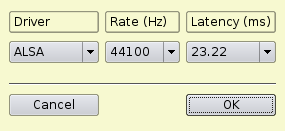
\includegraphics[width=0.5\textwidth]{images/sshot02.png}
 \caption{Der aktive Treiber kann in der Menüleiste ausgewählt werden. Traverso unterstützt ALSA, jack, und PortAudio, und hat einen \emph{Null Driver} für den Fall dass kein anderer Treiber verfügbar ist.}
 \label{fig_driverconf}
\end{figure}

\subsection{Port Audio}

\includegraphics[height=\baselineskip]{images/mac.png}

\includegraphics[height=\baselineskip]{images/win.png}
\\
Port Audio ist der empfohlene Treiber für Windows und Mac OS X verfügbar. Er bindet Traverso an das native Treibersystem der jeweiligen Plattform an. Die Samplerate und Latenzzeit können ebenfalls über die Menüleiste oder das Menü ,,Einstellungen $\rightarrow$ Einstellungen\dots $\rightarrow$ Audio Treiber'' konfiguriert werden.

\section{Aufnahme-Dateiformat}
Über das Menu ,,Einstellungen $\rightarrow$ Format der Aufnahmedateien'' kann ausgewählt werden, in welchem Format die aufgenommenen Audiodateien gespeichert werden sollen. \emph{Wave} ist seit Jahren der Standard für digitale Musik auf Computern. Die Daten werden unkomprimiert in 32-Bit-Auflösung gespeichert, unabhängig davon, welche Bit-Auflösung in der Treiber-Konfiguration eingestellt ist. Eine Einschränkung von Wave-Dateien ist jedoch die Begrenzung auf eine Dateigrö"se von maximal 2~GB. Für Mono-Dateien mit einer Auflösung von 44100~Hz und 32~Bit beträgt die maximale Aufnahmezeit etwa 3 Stunden und 20 Minuten. Für Stereo-Dateien sogar nur die Hälfte. Für längere Aufnahmen sollte daher das \emph{Wave-64}-Format verwendet werden, welches eine maximale Dateigrö"se jenseits aktueller Festplattengrö"sen bietet. Das dritte Format, \emph{WavPack}, verwendet einen verlustfreien Kompressionsalgorithmus, welcher die Dateigrö"se auf etwa die Hälfte eines unkomprimierten Formates reduziert. Die Komprimierung erfolgt jedoch in Echtzeit, was eine erhöhte Belastung des Prozessors, vor allem bei der Aufnahme, zur Folge hat. Mit einem schnellen Prozessor ist jedoch häufig der Gewinn an freiem Festplattenplatz und Platz auf Backup-Medien die bessere Wahl.
